\chapter{Imagerie radiale}
\setlength{\footskip}{50pt}
\label{Chap2}
\section{Description de l'espace de Fourier}

Une expérience de RMN standard, nous permet de mesurer un signal provenant d'un volume mais il est impossible d'assigner une position spatiale aux protons. Cependant, l'information spatiale peut être obtenue grâce à l'utilisation de gradient de champ magnétique supplémentaire. Le signal recueilli peut alors être stocké dans une matrice que l'on appelle espace de Fourier qui après une opération mathématique (transformée de Fourier) permettra d'obtenir une image. 
Généralement, la construction d'une image nécessite l'acquisition d'une série de données appelées acquisitions. Dans chaque acquisition, une impulsion de radiofréquence (RF) produit une nouvelle valeur d'aimantation transverse qui est alors échantillonnée selon une trajectoire particulière de l'espace de Fourier (figure \ref{fig:Signal2Image}).


\begin{figure}[h]
\centering
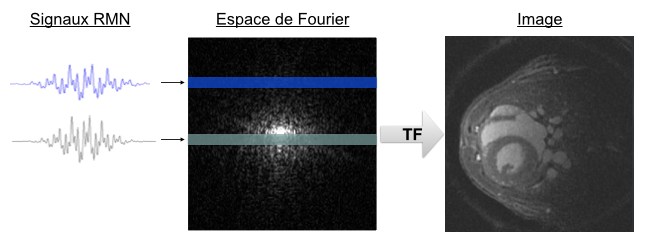
\includegraphics[scale=0.4]{./figure/chap2/Signal2Image.png}
\caption[Formation d'une image]{\label{fig:Signal2Image} Formation d'une image. }
\end{figure}

%V11 mars 2015. En principe, une image complète d'IRM peut être reconstruite à partir d'une seule acquisition en utilisant une trajectoire qui  parcoure tout l'espace de Fourier. C'est une méthode très souvent utilisé en imagerie fonctionnelle. Cependant, pour la plupart des applications cela entraine l'apparition d'artefacts dans l'image et d'une faible résolution spatial. Cela est due à la décroissance exponentielle du signal qui limite la fenêtre de temps d'acquisition exploitable. Mais cette fenêtre d'acquisition est aussi dicté par la performance du système de gradient et les contraintes physiologiques qui limite la vitesse à laquelle l'espace de Fourier peut être traversé. Il en résulte que la plupart des méthodes d'imagerie IRM utilisent de multiple acquisitions, chacune d'entre elles permettant de recueillir les informations d'une partie de l'espace de Fourier.

En principe, une image complète d'IRM peut être reconstruite à partir d'une seule acquisition en utilisant une trajectoire qui  parcoure tout l'espace de Fourier. Cependant, pour la plupart des applications cela entraine l'apparition d'artefacts dans l'image et d'une faible résolution spatial. Cela est due à la décroissance exponentielle du signal qui limite la fenêtre de temps d'acquisition exploitable. Mais cette fenêtre d'acquisition est aussi dicté par la performance du système de gradient et les contraintes physiologiques qui limite la vitesse à laquelle l'espace de Fourier peut être traversé. Il en résulte que la plupart des méthodes d'imagerie IRM utilisent de multiple acquisitions, chacune d'entre elles permettant de recueillir les informations d'une partie de l'espace de Fourier.

Une partie du développement de nouvelles méthodes d'acquisition en IRM correspond à modifier la stratégie et les trajectoires permettant de remplir l'espace de Fourier.


\subsection{Parcours de l'espace de Fourier}
\label{subsec:Parcours}

Un déplacement dans l'espace de Fourier s'effectue grâce à l'application des gradients de codage de l'espace. L'application d'un gradient induit une variation de la précession des spins dépendante de leurs positions dans l'espace. Lors de l'arrêt des gradients, les spins précessent à nouveau à la même fréquence mais ont accumulé une différence de phase (figure \ref{fig:ParcoursKspace}) qui peut se traduire par un déplacement dans l'espace de Fourier définie par :
\begin{equation}
k(t)= \frac{\gamma}{2\pi} \int_0^t G(s)ds
\end{equation}

\begin{figure}[h]
\centering
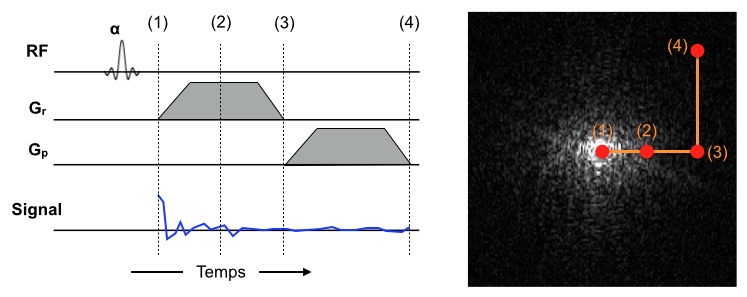
\includegraphics[scale=0.6]{./figure/chap2/ParcoursKspace.png}
\caption[Parcours de l'espace de Fourier]{\label{fig:ParcoursKspace} Le déplacement dans l'espace de fourier est proportionnel à l'aire des gradients utilisé. Les gradients sont limités par leurs amplitudes maximum, $G_{max}$, et leurs temps de monté, $S_{max}$, qui sont spécifique du système de gradient utilisé. Figure provenant extraite de la thèse du Dr. Lustig \cite{Lustig:2008ty}.}
\end{figure}

\subsection{Propriété de l'espace de Fourier}

L'espace de Fourier, de par sa nature, dispose de nombreuses propriétés qui peuvent être exploité lors du développement de nouvelles méthodes d'acquisition. 

\subsubsection{Régions centrales et extérieures}
\label{subsec:KSpaceRegion}
Les régions centrale et périphérique de l'espace de Fourier contribuent différemment à la construction de l'image. La figure \ref{fig:kSpaceResSig} illustre le fait que le centre de l'espace contient les informations de base fréquence de l'image correspondant principalement au signal et au contraste. Alors que la périphérie encode les hautes fréquences spatiales qui correspondent aux détails, au contour ainsi que le bruit.

\begin{figure}[H]
\centering
\includegraphics[scale=0.7]{./figure/chap2/kSpaceResSig.png}
\caption[Centre vs Extérieur]{\label{fig:kSpaceResSig} Les régions centrales et périphériques de l'espace de Fourier sont utilisées pour reconstruire les images. La reconstruction avec le centre de l'espace résulte en une image floue alors qu'avec l'extérieur on observe les contours des zones.}
\end{figure}

\subsubsection{Résolution et champ de vue}

La résolution de l'image est donné par la région de l'espace de Fourier qui est échantillonné, plus celle-ci est grande plus l'image sera résolue.
\begin{equation}
\Delta x = \frac{1}{2*k_{max}}
\end{equation}
où $k_{max}$ est la position du point échantillonnée la plus éloignée du centre de l'espace de Fourier. Le champ de vue est déterminé par la densité d'échantillonnage de cette région, Pour obtenir un plus grand FOV il faut échantillonner de manière plus dense l'espace de Fourier. La distance d'échantillonnage $\Delta k$  entre deux points en fonction du FOV est définie par :
\begin{equation}
\label{eq:FOV}
FOV = \frac{1}{\Delta k}
\end{equation}
Généralement, l'espace de Fourier est échantillonné de manière à respecter le critère de Nyquist qui dépend de la résolution spatiale et du champ de vue (FOV) désirés
\begin{equation}
\Delta k =\frac{2k_{max}}{n} \leq \frac{1}{FOV}
\end{equation}
où $n$ correspond au nombre de points échantillonnés pour une acquisition. Une violation du critère de Nyquist créera des artéfacts dans l'image dépendant du type de trajectoire utilisé pour échantillonner l'espace de Fourier (figure \ref{fig:Undersamp}).
\begin{figure}[H]
\centering
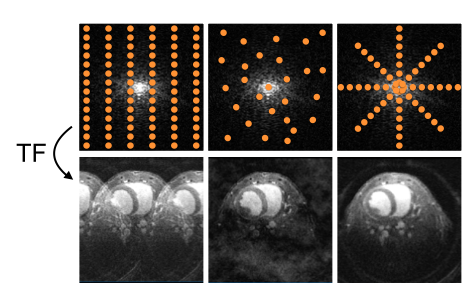
\includegraphics[scale=0.7]{./figure/chap2/Undersamp.png}
\caption[Sous-échantillonnage]{\label{fig:Undersamp} La résolution de l'image est dictée par l'étendue de l'espace de Fourier échantillonné. La violation du critère de Nyquist introduit des artéfacts dans le domaine image qui dépendent de la trajectoire utilisée. A gauche : Avec l'acquisition d'une ligne sur deux de l'espace, on observe des artéfacts de repliment. Au milieu : avec un espace sous-échantillonné aléatoirement avec un facteur 2, on observe des artéfacts incohérents. A droite : avec un espace sous-échantillonné 5 fois avec des trajectoires radiales, on observe une diminution de la résolution.}
\end{figure}

\subsection{Trajectoire d'échantillonnage}

\begin{figure}[h]
\centering
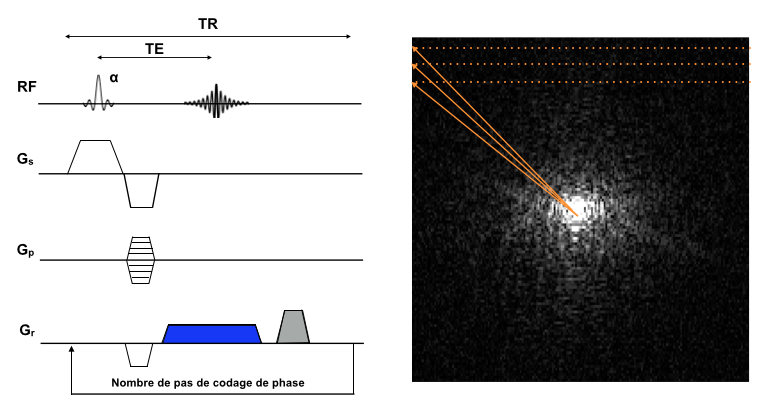
\includegraphics[scale=0.5]{./figure/chap2/TrajCart.png}
\caption[Trajectoire cartésienne]{\label{fig:TrajCart} Pour les trajectoires cartésiennes, la lecture du signal s'effectue durant l'application d'un gradient de lecture constant (selon $G_r$). Les autres gradients servant à positionner le premier point de la lecture après l'impulsion de radiofréquence $\alpha$.}
\end{figure}
La trajectoire la plus couramment utilisée est la trajectoire cartésienne qui consiste en l'acquisition de ligne parallèle de l'espace de Fourier (figure \ref{fig:TrajCart}). Cela s'explique par sa reconstruction extrêmement simple qui consiste en une Transformée de Fourier Rapide (FFT) selon chaque axe. Et surtout, la reconstruction à partir de cette trajectoire est peu sensible à de nombreuses sources d'imperfections. Le principal problème de ce shéma d'acquisition est sa sensibilité au mouvement et ses artéfacts cohérents de repliement qui sont crées en cas de sous-échantillonnage.
%%%%%Modif 08/03/2015
%Cependant, la conception d'une trajectoire est relativement libre et peut permettre d'obtenir certaines propriétés intéressante que ce soit en terme de temps, d'acquisition, faible sensibilité aux mouvement ou pour des applications spécifiques. 
Bien que ces schéma de trajectoires soient majoritairement employés, de nombreux autres ont été développés et sont décrit dans la littérature. Parmis ceux-ci, trajectoires radiales ont des propriétés intéressantes pour des applications sur le petit animal.


\section{Trajectoire radiale dans l'espace de Fourier}

\subsection{Principe}
Le schéma d'acquisition radial a tout d'abord été proposé par Lauterbur en 1973 \cite{lauterbur1973image}. Peu après l'introduction des scanners commerciaux, les trajectoires radiales ont été remplacé par des trajectoires cartésiennes car celles-ci étaient plus robuste aux hétérogénéités de champs $B_0$ et à la non-linéarité des gradients qui étaient très présents sur les premiers scanners IRM. Au fil des années, un intérêt s'est recréé pour les séquences radiales grâce aux progrès techniques en particulier sur la compensation des courants de Foucault dans les gradients et la meilleur homogénéité du champ statique. 

En imagerie radiale, le signal IRM est échantillonné selon des trajectoires suivant les rayons ou les diamètres d'un disque qui permettent d'obtenir respectivement une séquence à temps d'écho ultra-court (UTE) ou une séquence projection-reconstruction (PR). Dans le cas d'une séquence 2D la trajectoire est définie sur un disque et, pour les séquence 3D, sur une sphère. Les différentes trajectoires sont illustrées sur la figure \ref{fig:TrajRad}.

\begin{figure}[h]
\centering
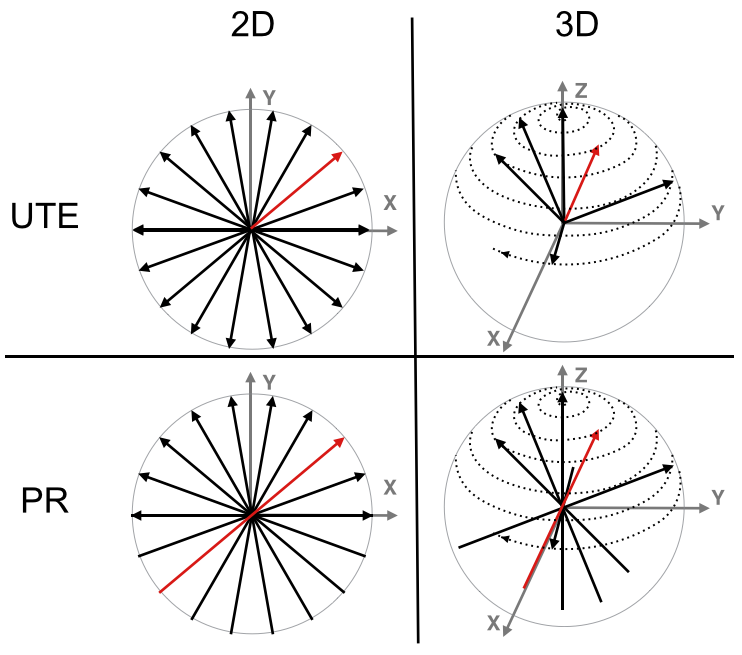
\includegraphics[scale=0.5]{./figure/chap2/TrajRad.png}
\caption[Trajectoires Radiales]{\label{fig:TrajRad} Trajectoire radiale 2D et 3D.}
\end{figure}




\subsection{Description mathématique}

Pour recueillir le signal selon les trajectoires radiales, l'amplitude des gradients varies selon les 3 axes simultanément selon l'équation :
\begin{equation}
\label{eq:AngleRadial}
\begin{split}
	G_x & =G\cos(\phi)\sin(\theta)\\
	G_y & =G\sin(\phi)\sin(\theta)\\	
	G_z & =G\cos(\theta)
\end{split}
\end{equation}
où $\theta$ et $\phi$ correspondent aux angles définies dans la figure \ref{fig:SphereCoord}.
Puisque les gradients dans les 3 directions sont utilisées pour chaque acquisition radiale de l'espace de Fourier, ils sont considéré comme des gradients de lecture plutôt que des gradients d'encodage de fréquence et de phase comme pour une acquisition cartésienne. Dans le cas d'une acquisition 2D, l'angle $\theta = \frac{\pi}{2}$ est utilisé ce qui a pour conséquence de ne faire varier les gradients que selon les axes x et y et de fixer la valeur du gradient z à 0.

Comme pour le cas cartésien, la distance entre deux points échantillonnés sur une projection est généralement définie par la taille du FOV désiré grâce à l'équation \ref{eq:FOV} et le nombre de points échantillonnés est définies par la résolution de base désirée $n$. Avec une trajectoire radiale, ces deux paramètres ne sont pas suffisant pour définir la résolution spatiale de l'image car celle-ci dépend aussi du nombre de projections $n_p$ utilisé. Pour satisfaire le critère de Nyquist, il est généralement suggéré dans la littérature \cite{bernstein2004handbook}  d'utiliser un nombre de projection égale à :
\begin{equation}
\label{eq:NyquistRad}
\begin{aligned}
	(2D)\;\;\;\; n_p = \frac{\pi}{2} \times n \\
	(3D)\;\ \ n_p = \pi \times n^2 
\end{aligned}
\end{equation}
qui assure que la distance entre deux points de projections voisines soit inférieure ou égale à $\Delta k$.
\begin{figure}
\centering
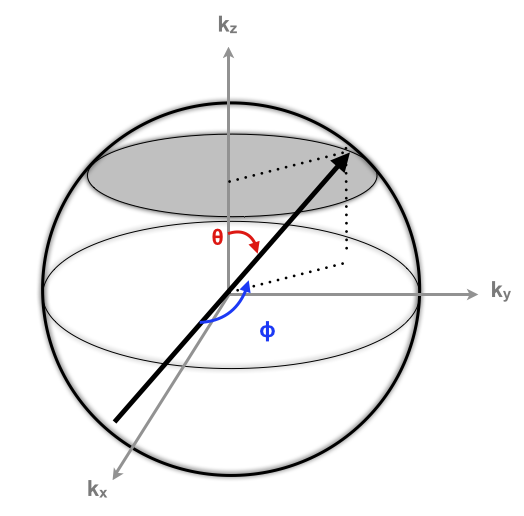
\includegraphics[scale=0.6]{./figure/chap2/SphereCoord.png}
\caption[Coordonnées sphériques]{\label{fig:SphereCoord} Représentation des angles $\theta$ et $\Phi$ utilisés  pour définir les trajectoires radiale en 3 dimensions.}
\end{figure}


\subsection{Chronogramme des séquences}

Comme décris dans la partie \ref{subsec:Parcours}, une trajectoire dans l'espace de Fourier correspond à l'application de gradient avec une intensité donné selon un ordre chronologique. Pour représenter une séquence il est courant d'utiliser un chronogramme qui représente les gradients de lecture $G_r$, de phase $G_p$ et de coupe $G_s$ ainsi que les impulsions RF.

\begin{figure}[h]
\centering
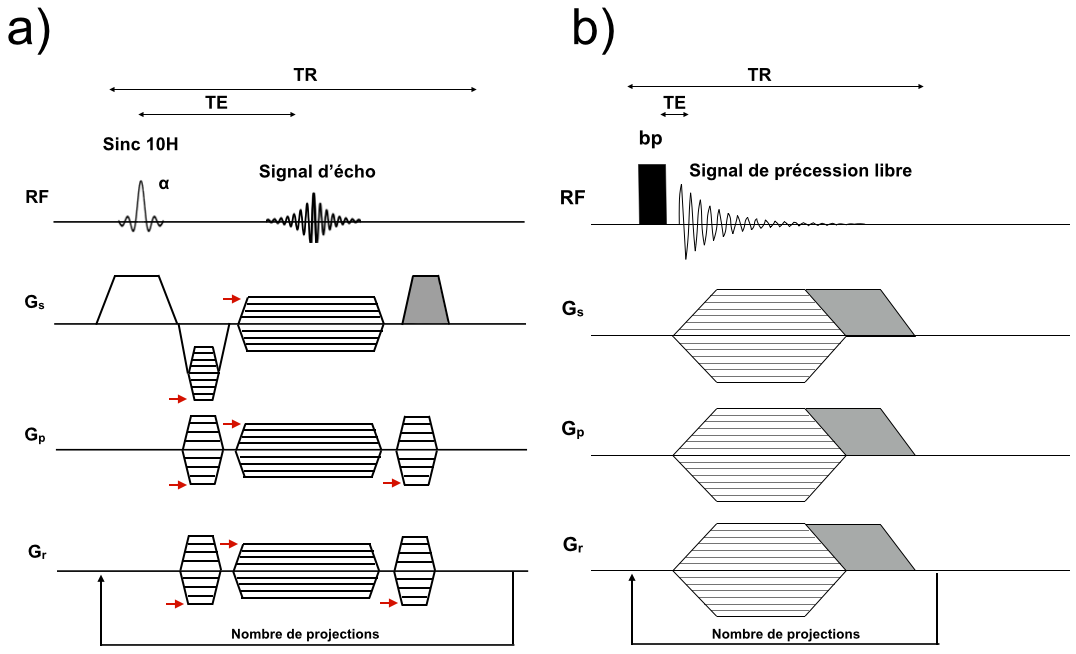
\includegraphics[scale=0.6]{./figure/chap2/KspacePR.png}
\caption[Coordonnées sphériques]{\label{fig:KspacePR} Gauche: chronogramme d'une séquence radiale 3D PR. Droite : Chronogramme d'une séquence radiale 3D UTE. Les gradients permettent de déphaser l'aimantation résultante avant la prochaine excitation de radiofréquence.} 
\end{figure}

Les chronogrammes de la séquence radiales 3D PR et UTE sont présentés dans la figure \ref{fig:KspacePR}. La séquence PR débute avec une impulsion RF qui peut être sélective grâce à l'application d'un  gradient selon l'axe $G_s$ suivi par un gradient de rephasage pour compensé l'évolution de phase indésirable causé par le gradient de sélection de coupe durant la seconde moitié de l'impulsion RF. Pour réduire la durée entre l'impulsion et la lecture du signal, les gradients de codage de l'espace sont appliqués en même que le gradient de rephasage de coupe pour amener dans une position périphérique de l'espace de Fourier. A partir de cette position, les gradients sont commutés avec une amplitude opposé de manière à parcourir l'espace en ligne droite selon un diamètre. Pendant ce déplacement, le signal est recueilli avec une fréquence d'échantillonnage fixe. La dernière étape de cette séquence consiste à déphasé l'aimantation restante avec des gradients de dephasage de type "spoiler". Pour chaque repetition, l'amplitude des gradients de déphasage puis de lecture sont modulés par l'équation \ref{eq:AngleRadial} pour définir les différentes trajectoires des projections.
La séquence UTE est similaire à la séquence PR mais ne disposent pas 
de gradient de sélection/rephasage de coupe, de gradient de codage de l'espace. La lecture s'effectuant au centre le signal recueilli est un signal de précession libre et non pas un signal d'écho.

Un autre type de séquence 3D radiale est très souvent utilisé que l'on appelle Stack-Of-Radial. Elle consiste en un empilement de plan contenant des trajectoires 2D UTE ou 2D PR. Le chronogramme de la séquence d'empilement UTE et la trajectoire correspondantes dans l'espace de Fourier sont présentées dans la figure \ref{fig:KspaceStackOfUTE}

\begin{figure}[H]
\centering
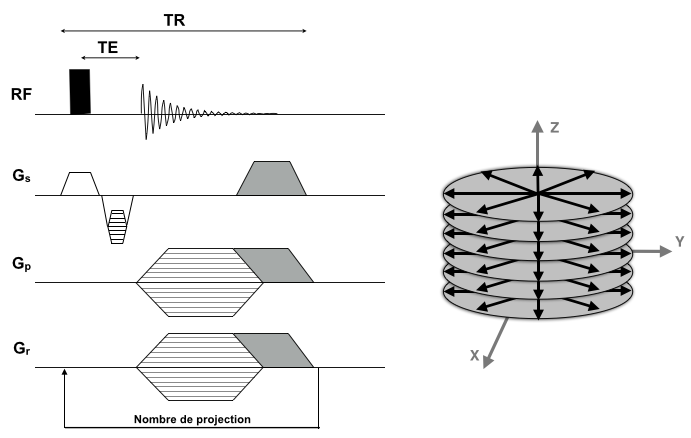
\includegraphics[scale=0.6]{./figure/chap2/KspaceStackOfUTE.png}
\caption[Coordonnées sphériques]{\label{fig:KspaceStackOfUTE} Droite : Trajectoire d'une séquence Stack-Of-UTE dans le plan de Fourier. Gauche : Chronogramme d'une séquence radiale Stack-Of-UTE.} 
\end{figure}

\subsection{Reconstruction}

\label{subsec:reconstruction}
Différentes approches sont utilisées pour la reconstruction des acquisitions radiales : Rétro-projection filtrée, gridding ou FFT non uniforme (nuFFT). Dans cette partie, je détaillerai la reconstruction par gridding qui est la plus communément utilisé et que j'ai appliqué durant ma thèse.

La méthode de reconstruction par remaillage (ou gridding) a été introduite en imagerie médicale par O'Sullivan en 1985 \cite{o1985fast} et fut plus tard appliqué à la reconstruction d'image IRM recueillit avec des trajectoires d'acquisitions non-cartésiennes. Cette technique consiste à interpoler les points échantillonnés sur une grille rectilinéaire avant d'effectuer une reconstruction avec une FFT (figure \ref{fig:Gridding}).

\begin{figure}[h]
\centering
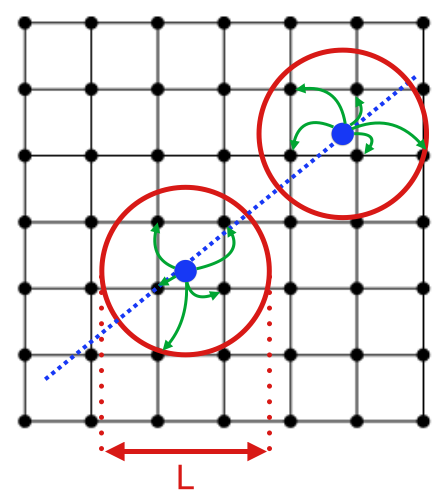
\includegraphics[scale=0.6]{./figure/chap2/Gridding.png}
\caption[Gridding]{\label{fig:Gridding} L'opération de gridding consiste à regarder quelles points de la grille cartésienne (en noir) sont contenues autour d'un point échantillonnés (en bleu) à une distance inférieur à $\frac{L}{2}$. La distance séparant chacun des points de la grille au point échantillonné est utilisée comme paramètre $d$ dans le kernel.} 
\end{figure}

Dans le cas de l'imagerie radiale, la densité de point variable dans l'espace de Fourier nécessite d'être compensé a priori ou a posteriori de l'interpolation. Généralement, la fonction de compensation en densité est utilisé comme un poids attribué à chaque point de l'espace de Fourier échantillonné. Pour redisposer les points sur une grille cartésienne, le signal mesuré est convolué avec un kernel d'interpolation. Le kernel Kaiser-Bessel a été prouvé comme étant optimal pour l'opération d'interpolation pour les acquisitions radiales. Celui-ci permet d'optenir des images de bonnes qualités avec une taille du kernel $L$ raisonnable et est défini par :
\begin{equation}
  K_{kb}(d) = \left\{
      \begin{aligned}
         \frac{1}{L}I_0(\beta \sqrt{1-(2d/L)^2}) \;\;\;\;\;\;  |d| \leq \frac{L}{2}\\
	     0 \;\;\;\;\;\; |d| \leq \frac{L}{2}
      \end{aligned}
    \right.
\end{equation}
où $L$ correspond à la taille du kernel, plus grand est sa taille plus l'image sera de bonne qualité cependant cela impactera fortement le temps de reconstruction pour un gain faible. une valeur de 2 à 4 est généralement utilisé permettant d'obtenir une image avec une bonne qualité tout en limitant le temps de reconstruction. $\beta$ est un facteur de forme  que l'on sélectionnera en accord avec l'équation décrite par Beatty et al. \cite{Beatty:2005fk}. $I_0$ correspond à la fonction de bessel modifiée de première d'espèce d'ordre 0. $d$ est la distance séparant le point à regridder au point de la grille. La forme du kernel est représenté dans la figure \ref{fig:KaiserBessel}.
\begin{figure}[H]
\centering
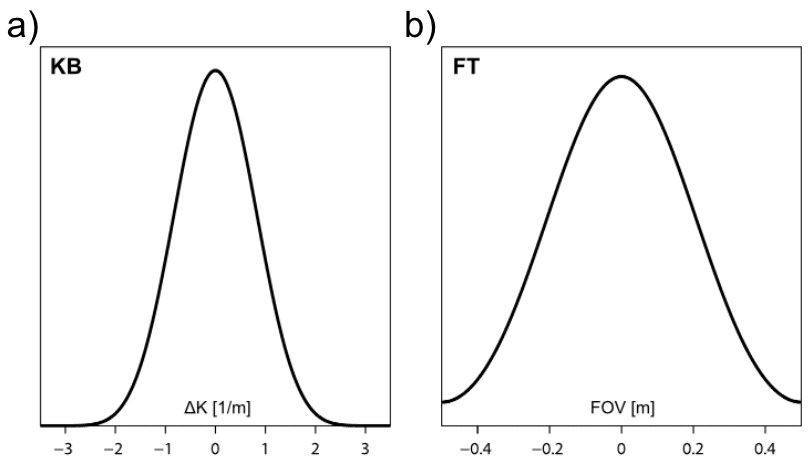
\includegraphics[scale=0.6]{./figure/chap2/KaiserBessel.png}
\caption[Kernel Kaiser-Bessel]{\label{fig:KaiserBessel} (gauche) Représentation du filtre kernel Kaiser-Bessel pour une valeur de $L = 6$ et $\beta = 13,8551$, où le FOV est normalisé à 1 m. (Droite) Transformée de Fourier du kernel.}
\end{figure}

A cause de la convolution avec un kernel ayant un taille fini, l'image obtenue après FFT montre des artéfacts de modulation appelé effet roll-off (figure \ref{fig:deapod}.
\begin{figure}[H]
\centering
\includegraphics[scale=0.6]{./figure/chap2/deapod.png}
\caption[Correction effet Roll-Off]{\label{fig:deapod} Effet de la correction de l'effet Roll-Off sur un fantôme. La variation de signal entre le centre et les bords du fantôme est compensé par la division avec la transformée de Fourier du kernel utilisé durant le gridding.}
\end{figure}
Cette modulation d'intensité de signal peut être compensé en divisant l'image par la transformée de Fourier du kernel qui est approximé par l'équation :
\begin{equation}
	FFT[K_{KB}](d) = \frac{\sin(\sqrt{(\pi L d)^2-\beta^2})}{\sqrt{(\pi L d)^2-\beta^2}}
\end{equation}
La convolution avec un kernel fini a aussi pour effet de créer des lobes secondaires qui sont repliés sur l'image.  Bien que l'amplitude initiale de ces lobes soient généralement faible avec un choix de kernel approprié, leurs intensités est amplifiées par la correction de l'effet roll-off. Une solution simple à ce problème est d'augmenter le champ de vue en effectuant le gridding sur une matrice plus grande, généralement 2 fois. L'augmentation du FOV est ensuite corrigé en n'utilisant que les pixels centraux correspondant au FOV utilisé.

La procédure de gridding se compose donc des étapes suivantes :
\begin{enumerate}
\item Compensation en densité
\item Interpolation sur une grille par convolution avec un kernel
\item FFT
\item Correction de l'effet roll-off
\item Découpe de l'image
\end{enumerate}

\subsection{Avantages et désavantages de la trajectoire radiale}

La trajectoire radiale offre des propriétés uniques du fait de sa géométrie ou de l'ordonnancement de l'acquisition de l'espace de Fourier. Certaines de ces propriétés sont avantageuses par rapport à une acquisition cartésiennes mais d'autres peuvent se transformer en inconvénients. Dans cette section, nous discuterons de ces propriétés en gardant en vue les applications possibles.
 
\subsubsection{Fonction d'étalement du point}

Pour comprendre les caractéristiques de n'importe quelle système d'imagerie, il est souvent très intéressant d'étudier la fonction d'étalement du point (PSF). La PSF décrit la réponse du système à une impulsion (un dirac) et permet de conclure sur comment un objet est imagé par celui-ci. En IRM, la PSF est fortement lié à la trajectoire dans l'espace de Fourier utilisée. En ignorant les phénomènes de relaxation pour plus de simplicité, la PSF d'une séquence IRM peut être obtenue en reconstruisant une image avec des données égale à 1 suivant la trajectoire radiale.

\begin{figure}[H]
\centering
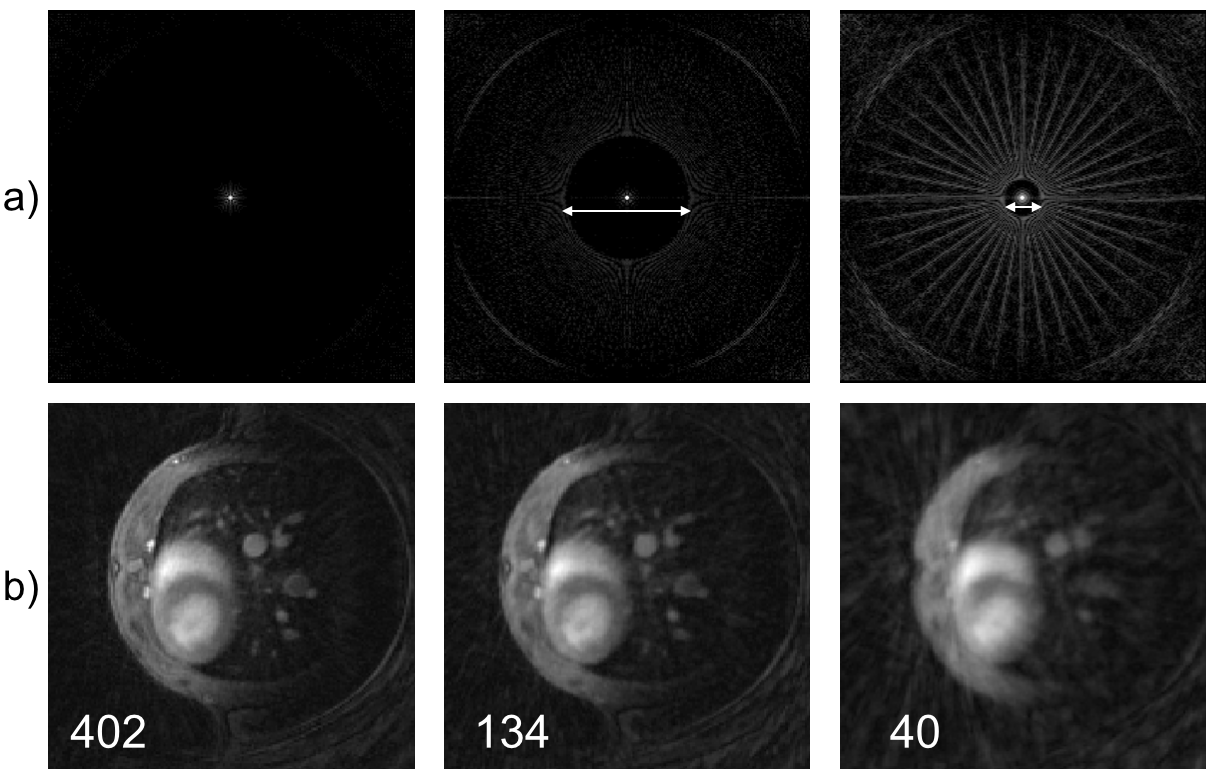
\includegraphics[scale=0.6]{./figure/chap2/PSF.png}
\caption[PSF]{\label{fig:PSF} PSF (haut) et la reconstruction correspondante (bas) obtenues sur un coeur de souris avec une trajectoire UTE 2D avec 402, 134 et 40 projections (résolution de base : 128 pixels). Les flèches blanches montrent le diamètre correspondant au champ de vue sans artéfacts.}
\end{figure}

La figure \ref{fig:PSF} montre des PSFs et leurs reconstructions correspondantes d'un cœur de souris obtenues avec une trajectoire radiale UTE avec une résolution de base de n = 128 pixels et différentes valeurs de projections $n_p$. D'après l'équation \ref{eq:NyquistRad}, pour la résolution de 128 pixels, il est nécessaire avec une acquisition UTE de recueillir 402 projections. Dans ce cas, on observe un pic au centre de la PSF bien distinct qui est entouré par des oscillations circulaires mineures qui diminuent en s'écartant du centre. Ces oscillations sont dues à l'utilisation d'un espace de Fourier fini, que l'on appelle aussi l'effet de troncature. Si l'on diminue le nombre de projection $n_p$ utilisé pour la reconstruction, par example à 134 projections,  on peut voir que, dans l'espace de Fourier, une limite se crée à une certaines distance qui délimite une région sans artéfact (Flèche blanche) \cite{Scheffler:1998fk} et que des artéfacts de "streaking" apparaissent en dehors de ce diamètre. De plus, la largeur à mi-hauteur du pic central est plus faible ce qui traduit une légère diminution de la résolution. Chaque "point" de l'objet étant convolué avec la PSF durant la reconstruction, le motif de "streaking" apparait sur l'image reconstruite à une distance correspondant à la taille de cette région sans artéfact dans la PSF. Lorsque l'on réduit le nombre de projection utilisé, le diamètre de cette région diminue et les artéfacts sont plus prononcés. Cela est particulièrement visible sur la PSF et l'image reconstruite avec 40 projections.
En 3D, les artéfacts de "streaking" sont plus diffus cela se traduit plutôt comme un bruit sur l'image ce qui permet un sous-échantillonnage de l'espace plus important \cite{Gu:2005aa}.

Par rapport à une trajectoire cartésienne, le nombre de ligne de l'espace de Fourier à recueillir est supérieure pour respecter le critère de Nyquist, ce qui augmente le temps d'acquisition requis pour les séquences radiales. En pratique, il est tout à fait possible de recueillir un nombre plus restreint de projection. Cela vient du fait que la région d'intérêt est souvent positionné à l'intérieur de l'objet donc que des artéfacts de "streaking" aux bords de l'image sont acceptable. Puisque le centre de la PSF est faiblement affecté par le nombre de projection utilisé, la trajectoire radiale offre une intéressante possibilité de sous-échantillonnage de l'espace de Fourier. Contrairement à l'acquisition cartésienne où une réduction du nombre de ligne recueillies aura pour conséquence une importante perte en résolution ou l'apparition d'artéfact de repliement qui rendent l'image inutile. Avec une trajectoire radiale, la plupart des informations restent visibles même avec une forte présence d'artéfact de "streaking".

\subsubsection{Distribution des points échantillonnés}

En imagerie radiale, puisque toutes les projections passent par le centre du plan de Fourier, le nombre de points échantillonnés est plus important pour les basses fréquences de l'espace de Fourier que pour les hautes fréquences. Cela est très différent des acquisitions cartésiennes où toutes les fréquences sont couvertes de la même façon. Bien que le fait d'avoir une distribution variable de points échantillonnés implique quelques difficultés pour la reconstruction (voir section \ref{subsec:reconstruction}), cela est une stratégie avantageuse pour la plupart des objets à imager. En effet, la plupart des images du monde réel sont caractérisées par une concentration en énergie près du centre de l'espace de Fourier, cela est vrai pour les images médicales de tomographie mais aussi pour les autres images naturelles \cite{srivastava2003advances}. C'est pourquoi il est intéressant de mesurer les basses fréquences plus "précisément" et n'avoir que moins de points échantillonnés dans les régions contenant moins d'information. 

Des images avec une faible résolution peuvent être reconstruite à partir d'une partie des projections recueillies. Cela est possible car le nombre de points échantillonnés est suffisamment dense au centre de l'espace de Fourier pour satisfaire le critère de Nyquist et obtenir une image sans artéfact comme expliqué dans la section précédente. De nombreuses applications peuvent être envisagée, par example en 2D, une série d'images résolues dans le temps peuvent être extraites d'un jeu de donnée complet pour identifier et corriger des artéfacts de mouvement qui peuvent survenir durant l'acquisition.

Une caractéristique supplémentaire de la géométrie radiale est que chaque projection apporte autant d'information sur les basses et hautes fréquences, alors qu'avec une trajectoire cartésienne les informations de basses fréquences ne sont contenues que dans quelques lignes. Cela fait de l'imagerie radiale une option attractive quand une mise à jour continu de l'image est importante, par example en imagerie interventionnelle (\cite{Peters:2004aa} ou bien pour de la prise de contraste dynamique \cite{Prieto:2010oq}). Récemment, une méthode alternative nommée "Highly Constrained Backprojection" utilise ce rafraichissement constant de l'image durant l'injection d'un agent de contraste avec une image ayant une haute résolution spatiale obtenues après le premier passage ce qui permet d'obtenir des valeurs de sous-échantillonnage très important et donc une forte résolution temporelle mais en gardant une bonne résolution spatiale \cite{Wu:2011vn,Grist:2012fk}.

\subsubsection{Mouvements et flux}
\label{subsec:MouvEtFlux}
L'avantage le plus important d'une acquisition radiale est sa faible sensibilité aux mouvements qui peut être expliqué par deux raisons. Premièrement, les séquences radiales sont principalement comparés avec les séquences cartésiennes qui sont extrêmement sensible aux mouvements. Cette sensibilité est une conséquence de la propriété de translation de la transformée de Fourier, un mouvement dans le domaine image se traduit par une modulation de la phase dans l'espace de Fourier. La forme de cette modulation dépend du type de mouvement et dans la littérature on distingue généralement des mouvements périodiques, pulsatiles et ayant une vitesse constante \cite{Glover:1992aa}. Bien que ces mouvements soient différents, ils causent tous l'apparition du même type d'artéfact qui sont des copies des parties mouvantes à d'autres positions dans l'image. Ces artéfacts apparaissent exclusivement dans la direction d'encodage de phase ou de coupe et selon le type de mouvement peuvent créer une ou plusieurs copies qui peuvent gêner l'interprétation. 

\begin{figure}[h]
\centering
\includegraphics[scale=0.5]{./figure/chap2/MotionArt.png}
\caption[Artéfact de mouvements]{\label{fig:MotionArt} Vue axiale des carotides d'une souris obtenue avec une séquence 3D PR à gauche et avec une séquence 3D cartésienne à droite. La flèche montre un artéfact de flux sur l'image cartésienne qui correspond à une copie de la crosse aortique.}
\end{figure}

En imagerie radiale, les artéfacts de mouvement se traduisent par du flou ou des artéfacts de "streaking" qui se propagent perpendiculairement à la direction de lecture et qui sont éloigné de l'objet en mouvement d'une certaine distance, ce qui disperse de manière plus homogène l'erreur. Cette dispersion est encore plus efficace pour les séquences radiales 3D que 2D. Ces artéfacts sont généralement moins dérangeant pour le diagnostique que les artéfacts apparaissant en imagerie cartésienne (figure \ref{fig:MotionArt}).
Deuxièmement, grâce au sur-échantillonnage du centre de l'espace de Fourier, il y a un moyennage des projections qui contrebalance les erreurs durant les phases de mouvement.
Ces deux propriétés réunies permette d'expliquer le fort engouement des séquences 3D radiale pour l'imagerie d'organes en mouvement ou de patient peu coopératif comme en pédiatrie \cite{block2014towards,Nayak:2014aa}.
Les séquences UTE bénéficient d'un autre avantage car, après l'excitation, les spins sont déphasés puis rephasé par moins de gradient qu'avec des séquences cartésiennes. Cela permet de limiter les artéfacts de déphasage de flux qui se traduise par une absence de signal (figure \ref{fig:FluxArt}).

Pour toutes ces raisons, l'utilisation de séquence radiale est un choix intéressant en particulier pour des applications en angiographie et sur le petit animal. 
\begin{figure}[H]
\centering
\includegraphics[scale=0.5]{./figure/chap2/FlowArt.png}
\caption[Artéfact de flux]{\label{fig:FluxArt} Vue coronale (en haut) et axiale (en bas) de la crosse aortique d'une souris obtenue avec une séquence 3D cartésienne à gauche et avec une séquence 3D Stack-Of-UTE à Droite. Les deux acquisitions ont été effectué sans synchronisation cardiaque ou respiratoire. La flèche épaisse montre une inhomogénéité du signal dans la crosse aortique qui sont des artéfacts de déphase du flux et les autres flèches  des artéfacts de mouvement}
\end{figure}

\subsubsection{Sur-échantillonnage en lecture}

Puisque l'espace de Fourier est échantillonné de manière discrète en IRM, la reconstruction de l'objet est périodique. C'est pour cela que l'on observe des effets de repliement de l'image si les points échantillonnés sont trop distant dans l'espace de Fourier et que les copies voisines se superpose dans le domaine image. Pour une résolution spatiale fixée, ce problème peut être éliminé en suréchantillonant la lecture. C'est à dire en utilisant une bande passante de réception plus grande, par example en la doublant, tout en gardant les mêmes valeurs de gradient. Cela permet donc d'augmenter le FOV mais aussi le nombre de point échantillonné d'un facteur 2 de manière à garder la même résolution spatiale. Cela permet aussi de compenser la diminution du SNR provenant de l'augmentation de la bande passante.

Pour l'imagerie cartésienne, cette méthode est limité à la direction de lecture car une réduction du nombre de points dans les autres directions demandera l'acquisition de lignes supplémentaires. Pour les cas radial, cette limitation n'existe pas et le sur-échantillonnage peut être employé dans toutes les directions. C'est une particularité particulièrement  intéressante pour l'imagerie de l'abdomen ou cardiac \cite{block2014towards,Johnson:2012uq} où les régions d'intérêts sont localisé au centre. Cela permet de réduire le FOV nécessaire et donc de réduire le temps d'acquisition nécessaire.

\begin{figure}[H]
\centering
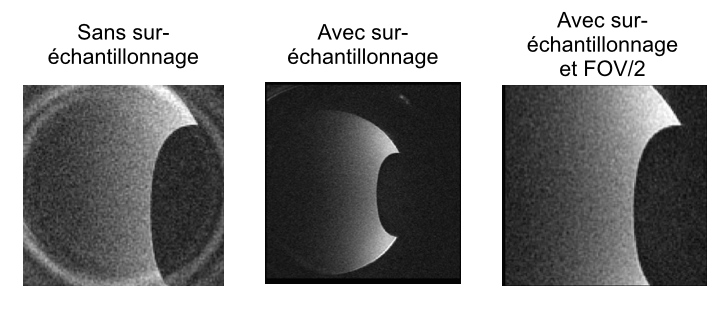
\includegraphics[scale=0.5]{./figure/chap2/Oversampling.png}
\caption[Artéfact de flux]{\label{fig:Oversampling} Vue axiale d'un fantôme. A gauche : Image acquise sans sur-échantillonnage (Nombre de points receuillies = 70 et bande passante de réception = 100 kHz). Au centre : Image acquise sans sur-échantillonnage (Nombre de points receuillies = 140 et bande passante de réception = 200 kHz). A droite : Image du centre coupé de manière à avoir la même dimension que celle de gauche. On observe que l'artéfacts en cercle n'est plus présent sur l'image avec sur-échantillonnage ainsi qu'une amélioration du SNR grâce à l'absence de repliement avec un FOV deux fois plus grand.}
\end{figure}

\subsubsection{Déviations des gradients}

Dans les séquence IRM, les gradients de champ magnétique doivent rapidement monter puis descendre en intensité à de multiples reprises ce qui implique la création de courants de Foucault dans les bobines. Cela va modifier la trajectoire d'échantillonnage des points dans l'espace de Fourier.
Pour les séquences cartésiennes, cela ne pose pas de problème majeur car des formes de gradients identiques sont générées dans la direction de lecture pour toutes les répétitions. Cela résultera durant la reconstruction à une translation de la position des points échantillonnées selon la direction de lecture et donc à une modulation de phase dans le domaine image qui disparaitra lorsque l'image en magnitude est calculé.

Cela est différent pour l'imagerie radiale car la direction de lecture varie pour chaque répétition. Dans cette situation, un simple délai de réponse des gradients cause une erreur non-uniforme de positionnement des points. Cela se traduit en des pertes de signal et du flou dans les images. C'est pour cela qu'il est nécessaire d'utiliser des méthodes de correction. Différentes techniques ont été proposé \cite{Alley:1998vn,Addy:2012kx} mais nous avons utilisé ici la méthode utilisé durant ma thèse originellement décrite par Zhang et al \cite{Zhang:1998uq}.
Celle-ci consiste à mesurer le signal dans deux coupes positionnées symétriquement par rapport au centre de l'image, perpendiculairement à la direction du gradient. La phase du signal est extraite du signal puis déroulée pour éviter les repliements. La trajectoire dans l'espace selon cette axe est alors calculée en utilisant la phase des deux coupes. Cette méthode est reproduite sur chaque axe pour obtenir les trajectoires dans la 2 ou 3 dimensions selon la séquence. Le chronogramme, la position des coupes et l'algorithme sont présentés dans la figure \ref{fig:SeqTraj}.

\begin{figure}[H]
\centering
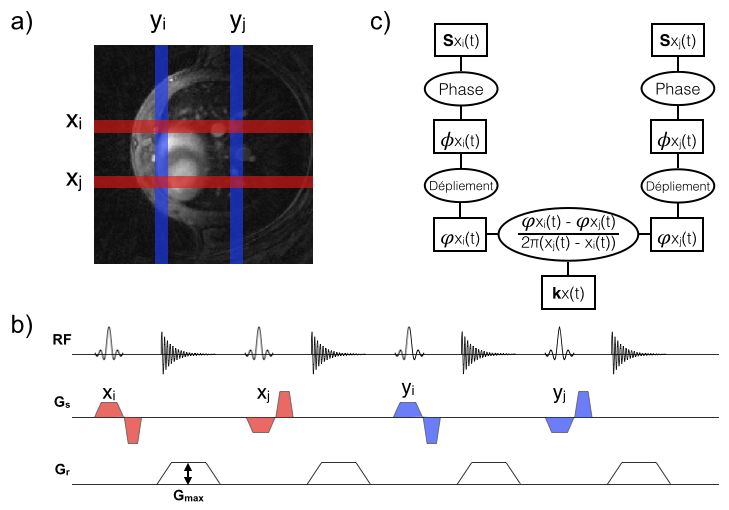
\includegraphics[scale=0.6]{./figure/chap2/SeqTraj.png}
\caption[Méthode mesure trajectoire]{\label{fig:SeqTraj}  
Mesure de trajectoire 2D UTE : (a) Positionnement des coupes de mesure symétrique par rapport à l'isocentre. (b) Chronogramme de la séquence utilisé. (c) Diagramme décrivant l'algorithme utilisé pour obtenir la trajectoire de l'axe verticale dans l'espace de Fourier à partir du signal dans les coupes $x_i$ et $x_j$.}
\end{figure}

\subsubsection{Sensibilité aux effets d'Off-Résonance}

En imagerie radiale les artéfacts d'off-résonance sont différents de ceux en imagerie cartésienne. La variation d'évolution de la phase cause un déplacement des informations spatiale selon chaque orientation des projections qui crée donc un flou dans l'image (figure \ref{fig:OffRes}).
On peut distinguer plusieurs sources d'artéfacts (la graisse, les effets de susceptibilité, l'inhomogénéité du champ statique, etc). La correction de ces artéfacts a postériori n'est pas triviale et une stratégie plus rationnelle consiste à les réduire en modifiant la méthode d'acquisition avec :
\begin{enumerate}
\item Une augmentation de la bande passante de réception
\item L'utilisation de séquence à temps d'écho court
\item L'utilisation de séquence de type Echo de Spin
\end{enumerate}

Généralement, la principale source d'artéfact d'off-résonance est la présence de graisse. En imagerie cardio-vasculaire sur petit animal la graisse est peu présente autour des zones d'intérêts comme le cœur, la crosse aortique ou les carotides ce qui limite les artéfacts. Cependant pour des méthodes demandant de long temps d'écho, par example, pour obtenir un contrast $T_2^*$, l'imagerie radiale n'est pas conseillé et une approche cartésienne est préférable ou bien l'utilisation obligatoire d'une méthode de suppression de graisse (saturation, excitation sélective etc).
\begin{figure}[H]
\centering
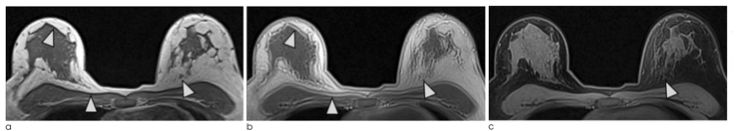
\includegraphics[scale=0.7]{./figure/chap2/OffRes.png}
\caption[Artéfact d'Off-résonance]{\label{fig:OffRes}  
(a) En imagerie cartésienne, la présence de graisse crée un artéfact de déplacement chimique dans la direction de lecture. (b) A cause de la modification de l'orientation de la direction de lecture en imagerie radiale, les artéfacts apparaissent comme un floue entourant les zones graisseuses. (c) Ces artéfacts peuvent être éliminé en utilisant une méthode de suppression de graisse.Figure extraite de Block et Al. (JKSMRM 2014)}
\end{figure}

\section{Résumé}

Avec un schéma d'acquisition radiale, les données de l'espace de Fourier sont recueillies selon des projections plutôt que des lignes parallèles. La modification d'une séquence cartésiennes existantes en une séquence radiale peut généralement être facilement effectuée que ce soit en 2D ou en 3D. Cependant, à cause de la position non équidistante des points, une méthode de reconstruction spéciale doit être utilisée comme le regridding.

L'imagerie radiale dispose de plusieurs avantages par rapport à une acquisition cartésienne comme une faible sensibilité aux artéfacts de flux et de mouvement, la possibilité de sur-échantillonner l'acquisition dans toutes les directions sans augmenter le temps d'acquisition requis ce qui élimine les artéfacts de repliement. De plus, le centre de l'espace de Fourier est sur-échantillonné, ce qui amène un intéressant comportement lors du sous-échantillonnage de l'acquisition. Bien que l'acquisition de moins de projections puissent créer des artéfacts de "streaking", une grand partie des informations de l'objet reste visible même avec un fort facteur d'accélération, ce qui n'est pas le cas avec une trajectoire cartésienne. De plus, chaque projection acquière un niveau équivalent d'information de haute et de basse fréquences, ce qui offre une mise-à-jour des informations plus homogène pour des applications en temps réelle ou dynamique en IRM.

D'un autre côté, le nombre de projection à recueillir pour obtenir un espace de Fourier complet est plus important qu'en imagerie cartésienne ce qui peut prolonger le temps d'acquisition. L'imagerie radiale est aussi plus sensible aux déviations des valeurs des gradients, bien qu'aujourd'hui cela soit un problème moins important avec les systèmes récents d'IRM. Le principale problème de cette méthode est sa sensibilité aux artéfacts de déphasage et en particulier de déplacement chimique. C'est pourquoi l'utilisation de séquence radiale n'est pas recommandé pour obtenir un contraste $T_2^*$.

